\documentclass{beamer}
\usepackage{lmodern}

\title{SIAM-IMA Etymo workshop - keyword extraction}
\author{Steven Elsworth}
\date{June 13, 2018}

\begin{document}
\maketitle

\begin{frame}
 \frametitle{\centerline{Keyword extraction}}
Overview of problem, given txt, find keywords
\end{frame}

\begin{frame}
\frametitle{Previous Approaches}
\begin{itemize}
\item Machine Learning
\item TFIDF
\item RAKE
\item Graph Based Approaches
\end{itemize}
\end{frame}

\begin{frame}
\frametitle{Machine Learning}
\end{frame}

\begin{frame}
\frametitle{TFIDF: Term Frequency, Inverse Document Frequency}
\end{frame}

\begin{frame}
\frametitle{RAKE: Rapid Automatic Keyword Extraction}
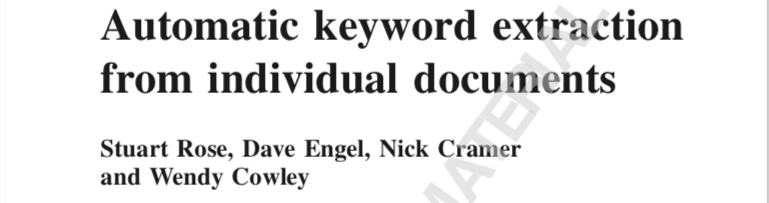
\includegraphics[width= \textwidth]{img/RAKE}
\vspace{1cm}
'An unsupervised, domain-independent, and language-independent method for extracting keywords from individual documents'
\vspace{0.5cm}

'The input parameters for RAKE comprise a list of stop words (or stoplist), a set of phrase delimiters, and a set of word delimiters.'
\end{frame}

\begin{frame}
\frametitle{RAKE Example}
\begin{itemize}
\item \textbf{Document:} \color{red} what example should we use? \color{black}
\vspace{0.3cm}
\item \textbf{Stop words:} Fox, Christopher. "A stop list for general text." ACM SIGIR Forum. Vol. 24. No. 1-2. ACM, 1989.
\vspace{0.3cm}
Example = ' a, about, above, across, after, again, against, all, almost, alone, along, already, also, although, always, among, an, ...'
\item \textbf{Phrase delimiters:} '.', ',', '!', ':', ';'
\vspace{0.3cm}
\item \textbf{Word delimiters:} ' ', '  ', '   ', '    ', '     ', ...
\end{itemize}
\end{frame}

\begin{frame}
\frametitle{RAKE: Extracted Keywords}

list extracted keywords

explain scorings
\end{frame}

\begin{frame}
\frametitle{Graph Based Approach}
\end{frame}

\end{document}
